

\documentclass{article}

\usepackage{fancyhdr} % Required for custom headers
\usepackage[utf8]{inputenc}
\usepackage{lastpage} % Required to determine the last page for the footer
\usepackage{extramarks} % Required for headers and footers
\usepackage[usenames,dvipsnames]{color} % Required for custom colors
\usepackage{graphicx} % Required to insert images
\usepackage{listings} % Required for insertion of code
\usepackage{courier} % Required for the courier font
\usepackage{lipsum} % Used for inserting dummy 'Lorem ipsum' text into the template
\usepackage{multirow}
\usepackage{ulem}

% Margins
\topmargin=-0.45in
\evensidemargin=0in
\oddsidemargin=0in
\textwidth=6.5in
\textheight=9.0in
\headsep=0.25in

\linespread{1.1} % Line spacing

% Set up the header and footer
\pagestyle{fancy}
\lhead{\authorName} % Top left header
\chead{\exClass: \exTitle} % Top center head
\rhead{\firstxmark} % Top right header
\lfoot{\lastxmark} % Bottom left footer
\cfoot{} % Bottom center footer
\rfoot{Page\ \thepage\ of\ \protect\pageref{LastPage}} % Bottom right footer
\renewcommand\headrulewidth{0.4pt} % Size of the header rule
\renewcommand\footrulewidth{0.4pt} % Size of the footer rule

\setlength\parindent{0pt} % Removes all indentation from paragraphs

% variables
\newcommand{\exTitle}{Problem set 4} % Assignment title
\newcommand{\exDueDate}{February\ 17,\ 2014} % Due date
\newcommand{\exClass}{TMA4280} % Course/class
\newcommand{\authorName}{Håkon Åmdal} % Your name

%----------------------------------------------------------------------------------------
%	TITLE PAGE
%----------------------------------------------------------------------------------------

\title{
\vspace{2in}
\textmd{\textbf{\exClass:\ \exTitle}}\\
\normalsize\vspace{0.1in}\small{Due\ on\ \exDueDate}\\
\vspace{3in}
}

\author{\textbf{\authorName}}
\date{} % Insert date here if you want it to appear below your name

%----------------------------------------------------------------------------------------

\begin{document}

\maketitle
\newpage

I will not have a thorough explanation of the code in this document, as it is well structured and well commented. The source code contains the following files:
\begin{itemize}
	\item \emph{ps4.c} - Code for solving the specific problem.
	\item \emph{util.c} - Utlity library.
	\item \emph{CMakeLists.txt} - CMake file which lets the user chose wheter to compile with OpenMP and/or MPI support.
\end{itemize}

\paragraph{OpenMP}
In order to utilize OpenMP, pragma commands was added to the loop filling up the series and the one summing the series.

\begin{figure}[h]
	\centering
	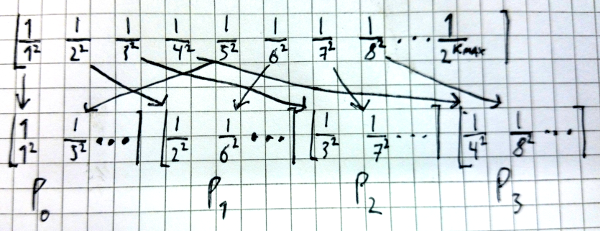
\includegraphics[width=8cm]{img/node_distribute.png}
	\caption{Distributing the series to four nodes}
	\label{fig:node_distribute}
\end{figure}
\paragraph{MPI}
To use the MPI library, size and rank variables were introduced, in order to manage the program flow with multiple processors. The initial series vector then had to be filled in a different way. A function to partially fill up the vector was made, a function that required the number of parts the original vector is to be split up in and the offset.  With four nodes, the first node would get element 0, 4, 8, 12... and the second would get element 1, 5, 9, 13... Please see figure \ref{fig:node_distribute}. This distribution algorithm works without side effects as long as the number of nodes is a power of 2 and less than $2^{K_{max}}$.
\\
\\ Here is a list of MPI calls used, excluding initialization and finalization calls:
\begin{itemize}
	\item \emph{MPI\_Send} - Used by node 0 to send out the partial series buffer to the other nodes, one node at a time.
	\item \emph{MPI\_Recv} - Used for all the other nodes to receive their partial series from node 0.
	\item \emph{MPI\_Reduce} - Used on every iteration for a $k$ value. Each node will calculate the sum of a part of their series, and the result will (by MPI's help) be reduced and end up at node 0.
\end{itemize}

\paragraph{Enabling and disabling libraries}
OpenMP and MPI can both individually be turned on and off. If MPI support is turned off, the preprocessor conveniently makes sure that no MPI dependencies are sent to the compiler, making the program compile and run on machines with no MPI. The program have been tested and verified to work with both OpenMP and MPI enabled simultaneously.
\begin{figure}[h]
	\centering
\begin{tabular}{c | c c c c}
	\hline
	k & Single Processor & P = 2 & P = 8 & P = 16 \\
	\hline
	\hline
	3 	& 1.175120e-01 & 1.175120e-01 & 1.175120e-01 & 1.644934e+00 \\
	4 	& 6.058753e-02 & 6.058753e-02 & 6.058753e-02 & 6.058753e-02 \\
	5 	& 3.076680e-02 & 3.076680e-02 & 3.076680e-02 & 3.076680e-02 \\
	6	& 1.550357e-02 & 1.550357e-02 & 1.550357e-02 & 1.550357e-02 \\
	7	& 7.782062e-03 & 7.782062e-03 & 7.782062e-03 & 7.782062e-03 \\
	8	& 3.898631e-03 & 3.898631e-03 & 3.898631e-03 & 3.898631e-03 \\
	9	& 1.951219e-03 & 1.951219e-03 & 1.951219e-03 & 1.951219e-03 \\
	10	& 9.760858e-04 & 9.760858e-04 & 9.760858e-04 & 9.760858e-04 \\
	11	& 4.881621e-04 & 4.881621e-04 & 4.881621e-04 & 4.881621e-04 \\
	12	& 2.441108e-04 & 2.441108e-04 & 2.441108e-04 & 2.441108e-04 \\
	13	& 1.220629e-04 & 1.220629e-04 & 1.220629e-04 & 1.220629e-04 \\
	14	& 6.103329e-05 & 6.103329e-05 & 6.103329e-05 & 6.103329e-05 \\
	\hline
	
\end{tabular}
\caption{Results with different number of nodes}
\label{fig:results}
\end{figure}

\paragraph{Running with different numbers of processors}
As seen in figure \ref{fig:results}, the results of running with $P=1$, $P=2$ and $P=8$ are all the same, as it should be. This is not the case for $P=16$, when $k=3$, the resulting sum equals $0.0$. Acutally, the program will not run correctly for passes where $2^k \le P$ because of integer division. If $P=16$ and $2^k=8$, each node will theoretically need to calculate $0.5$ of the elements. This is rounded down, so that each node will report the sum of $0.0$. I have done no effort in trying to correct this issue, because if the series is smaller than the number of nodes, the value of $P$ is probably a real overkill (and could easily be set to a lower value).

\paragraph{Memory requirement}
Neglecting other variables ($n >> 1$), we can in the source code see that each processor will allocate space for no more than $n \over P$ floating point values with double precision. $P_0$ will use its own partial vector buffer when using \emph{MPI\_Send}, and when done, use the same buffer for it's own values. With a total of $P$ processors, we get the following memory equation:
\begin{equation}
	M = O(P \times {n \over P} ) = O(n)
\end{equation}

\paragraph{Floating point operations to fill up a vector}
In the loop filling up the partial vector, a total of 2 additions, 2 multiplications, 1 division and 1 increment are performed. This loop is run the same amount of times as $2^{K_{max}}$:
\begin{equation}
	F_{fill} = 6 \times 2^{K_{max}}
\end{equation}
With $K_{max}=14$ this equals $98'304$ floating point operations.


\paragraph{Floating point operations to calculate the sum}
Each node will individually perform $F_{node}$ additions:
\begin{equation}
	F_{node} = {2^{K_{max}} \over P} - 1
\end{equation}
The MPI allreduce will add together a total of $P-1$ partial sums. From this, we get:
\begin{equation}
	F_{sum} = P({2^{K_{max}} \over P} - 1) + P -1 = (2^{K_{max}} - P) + P -1 = 2^{K_{max}} - 1
\end{equation}

With $K_{max}=14$ this equals $16'383$ floating point operations.



\paragraph{Load balancing}
The multi-processor program is not balanced, because $P_0$ is the only processor generating any elements. As we can see from above calculations, generating the vector requires much more floating point operations than summing the elements together. This task should also be split to different processors in order to load balance the program.

\begin{figure}[t]
\centering
\begin{tabular}{c | c c c c}
	\hline
	$K_{max}$ & No OpenMP, no MPI & OpenMP, no MPI & OpenMP, P=2 & OpenMP, P=4 \\
	\hline
	\hline
	14	& 2.369881e-04 & 4.323812e-03 & 8.273387e-02 & 2.003469e-01 \\
	29 	& 2.775124e+00	& 1.254882e+00	& 1.706845e+00 & 1.821380e+00 \\
\end{tabular}
	\caption{Running times with various parallelization techniques on an Intel Core i7-3612QM 2.1GHz}
	\label{fig:time}
\end{figure}
\paragraph{Parallel processing or not?} I think parallell processing is very attractive for calculating sums in general, but the problem size in this exercise is to small, making the overhead too big. I have performed a very informal and non-scientific performance test on the run times, as shown in figure \ref{fig:time}. We can see that for $K_{max}=1$, the non parallel program runs one order of magnitude faster than the OpenMP version. Increasing $K_{max}$ to 29, will make the OpenMP run twice as fast as the serial one.


\paragraph{Conventions}
As I have never touched the C programming language before, I have tried to read myself up on some standards and style for coding in this language. I have followed a document\footnote{http://www.jetcafe.org/jim/c-style.html} written by Jim Larson in 1996, as it seemed well rationalized. 

\end{document}

